\subsection{Data} \label{subsec:data}
% TODO wieso habe ich diese Datasets gewählt? Ehr Abgrenzung?
% TODO Warum habe ich TPM wert genommen?

Our study consists of two main datasets.
One includes healthy tissue data from the Genotype-Tissue Expression (GTEx) project,
and the other includes cancerous tissue data from the Cell Model Passport (CMP) project.
These two datasets are the base for the gene nodes in our graph database.
For these, we need to have a single table with each gene as row and a single value for healthy and cancerous TPM values for every gene in every tissue.
To have an identifier for every gene, we use the Ensemble ID (ENS ID) as the primary key for the gene nodes.
These are unique id for genes, proteins and other genetic elements collected in the Ensemble database
from 1999 by the European Bioinformatics Institute and the Wellcome Trust Sanger Institute~\cite{ensembl_project}.
\\


% Genotype-Tissue Expression (GTEx) dataset
For the healthy tissue samples used in this study,
we utilized the $"$GTEx\_Analysis\_2017-06-05\_v8\_\newline
RNASeQCv1.1.9\_gene\_tpm$"$ dataset from the GTEx portal~\cite{gtex_download}.
The \textbf{GTEx portal} is a large-scale, publicly available resource for studying gene activity.
The Adult GTEx project aims to characterize the gene expression patterns in healthy tissues across different individuals and ages,
providing valuable insights into the underlying biology of human development and disease.
This dataset is part of the Bulk Tissue Expression data in the V8 release,
which provides RNA sequencing data for a large number of tissue samples.
% genommen weil in der Wissenschaft üblich
The used dataset is in a .gct file format that contains TPM values for 56,156 genes identified by ENS ID as rows in 17,382 different tissues as columns.
The data was initially stored in a file in wide format where each tissue had its own column.
% TODO more?
The TPM values for the tissues are between 0 and 747,400.
Since there are no missing values in the dataset, we did not need to handle any missing data.
To process this data into a suitable format, we employed the following steps:
\begin{enumerate}
    \item \textbf{Reshaping to length format:} We read the data from the original file in chunks of 3,000 rows at a time to avoid memory issues.
    For each chunk of data, we transformed the columns for each tissue into individual rows,
    resulting in a dataset with three columns and 56,156 * 17,382 rows.
    \item \textbf{Grouping by genes:} Once all chunks had been processed, we separated the combined dataset in new chunks of approximately 200 million rows.
    These chunks have been grouped by gene using an aggregate function that calculated both the sum and count of TPM values for each gene.
    \item \textbf{Calculating mean TPM:} To handle genes that had been split across multiple chunks,
    we performed a global aggregation on the genes of the sum of the dataset.
    We then calculated the mean TPM value for each gene by dividing the sum by the count of each observation.
    %TODO unklar
\end{enumerate}
The resulting dataset~\ref{fig:03_01_df_GTEX_healthy_mean} with 56,156 genes and a mean TPM value for every gene was saved as a CSV file for further processing.\\

\begin{table}[h]
    \centering
    \caption{GTEx processing steps }\label{tab:gtex_table}
    \resizebox{\textwidth}{!}{
    \begin{tabular}{|c|c|c|c|}
        \hline
        \textbf{Original Format} & \textbf{Reshaping to length format} & \textbf{Grouping by genes} & \textbf{Calculating mean TPM} \\
        \hline
        & & & \\[1mm] % adding more space to the row
        %TODO rewrite to other format - force linebreak
        $\begin{bmatrix}
            i \text{ - number of genes} \\
            j \text{ - number of tissues} \\
            a_{ij} \text{ - TPM value for gene i in tissue j} \\
        \end{bmatrix} $ &
        $ A_{\text{long}} = (\text{Gen}_i, \text{Tissue}_j, a_{ij}) $ &
        $ A_{\text{agg}} = (\text{Gen}_i, S_i, C_i )$ &
        $ A_{\text{mean}} = (\text{Gen}_i, M_i )$ \\

        & & & \\[1mm] % adding more space to the row
        & & $ S_i = \sum_{j=1}^{j} a_{ij}, \quad C_i = \sum_{j=1}^{j} 1 $ &
        $ M_i = \frac{S_i}{C_i} $ \\

        & & & \\[1mm] % adding more space to the row

        $ A = \begin{bmatrix}
            a_{11} & a_{12} & \dots & a_{1j} \\
            a_{21} & a_{22} & \dots & a_{2j} \\
            \vdots & \vdots & \ddots & \vdots \\
            a_{i1} & a_{i2} & \dots & a_{ij}
        \end{bmatrix} $ &

        $ A_{\text{long}} = \begin{bmatrix}
            \text{Gen}_1 & \text{Tissue}_1 & a_{11} \\
            \text{Gen}_1 & \text{Tissue}_2 & a_{12} \\
            \vdots & \vdots & \vdots \\
            \text{Gen}_i & \text{Tissue}_j & a_{ij}
        \end{bmatrix} $ &

        $ A_{\text{agg}} = \begin{bmatrix}
            \text{Gen}_1 & S_{1} & C_{1} \\
            \text{Gen}_2 & S_{2} & C_{2} \\
            \vdots & \vdots & \vdots \\
            \text{Gen}_i & S_{i} & C_{i} \\
        \end{bmatrix} $ &

        $ A_{\text{mean}} = \begin{bmatrix}
            \text{Gen}_1 & M_{1}\\
            \text{Gen}_2 & M_{2} \\
            \vdots & \vdots\\
            \text{Gen}_i & M_{i}\\
        \end{bmatrix} $ \\

        & & & \\[1mm] % adding more space to the row
        \hline
        & & & \\[1mm] % adding more space to the row

        % Example Matrix Representation
        $ A = \begin{bmatrix}
            %\text{GTEX-1117F} & \text{GTEX-1122O} & \text{GTEX-113IC} \\
            8.764 & 0.07187 & 3.215
        \end{bmatrix}$ &

        $ A_{\text{long}} = \begin{bmatrix}
            \text{ENSG...938} & \text{GTEX-111...} & 8.764 \\
            \text{ENSG...938} & \text{GTEX-112...} & 0.07187 \\
            \text{ENSG...938} & \text{GTEX-113...} & 3.215
        \end{bmatrix}$ &

        $ A_{\text{agg}} = \begin{bmatrix}
            \text{ENSG...938} & 12.051 & 3
        \end{bmatrix}$ &

        $ A_{\text{mean}} = \begin{bmatrix}
            \text{ENSG...938} & 4.017
        \end{bmatrix}$ \\

        & & & \\[1mm] % adding more space to the row
        \hline
    \end{tabular}
    }
\end{table}

\begin{figure}[h]
    \centering
    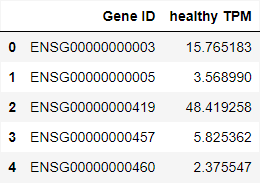
\includegraphics[height=\dfheight]{figures/03_01_GTEX_healthy_mean}
    \caption{Example data of processed Genotype-Tissue Expression dataset}
    \label{fig:03_01_df_GTEX_healthy_mean}
\end{figure}




% Cell Model Passport
For the analysis of gene activity in lung cancer, we utilized data from the \textbf{Cell Model Passport (CMP) project},
a comprehensive resource for studying cancer-related gene expression.
% TODO wirte more about The CMP project...

We obtained the dataset from the CMP portal~\cite{cmp_download}, specifically the $"$Expression Data$"$ section,
with the name \texttt{rnaseq\_all\_data\_20220624}.
This dataset contains data from the Sanger Institute and the Broad Institute and
consists of a large CSV file containing TPM values for genes associated with diverse cancer types, including lung cancer.
Initially, the data was stored in long format with columns for CMP IDs for genes, tissues, TPM values, and additional information.
To focus on lung cancer-specific data, we loaded an additional file containing model annotations. \cite{cmp_tissue_models}
We then filtered the CMP dataset to include only models from the annotation file with lung cancer as the cancer type.

The resulting dataset comprises 7,564,389 rows containing genes and tissues with associated TPM values for lung cancer.
Specifically, the dataset includes information on 37,262 unique genes across 203 distinct tissue types.
Notably, this dataset is free from missing values, and the TPM values span a wide range of 0 and 132,676.

To prepare the data for further processing, we performed the following steps:
\begin{enumerate}
    \item \textbf{Grouping by genes:} We grouped the dataset by genes to obtain a mean TPM value for every gene.
    This step involved aggregating the data by gene names, resulting in a new dataset with a mean TPM value for each gene.
    \item \textbf{Adding ENS ID:}
    The original dataset contained only CMP ID per gene but lacked the universal Ensembl ID required for matching genes across datasets.
    To address this limitation, we needed to add corresponding Ensembl IDs to our genes using their gene\_symbol.
    For this purpose we downloaded an Ensemble file from biomart~\cite{bio_marts},
    which contains the ENS ID and gene\_symbol.

    By analyzing the file, we encountered an issue where some gene\_symbols were not unique in the Ensemble file.
    To resolve this problem, we dropped all rows with duplicate gene\_symbols. %, which reduced the number of rows in the Ensemble file by a significant amount. % 10.605/48.311 rows
    We then merged the Ensemble table with our CMP data on gene\_symbols to retrieve the ENS IDs for each gene.

    \item \textbf{Removing missing ENS ID:} After merging the data, we found that 3,760 genes had no ENS ID associated with them.
    Since these genes were likely duplicates or did not exist in the Ensemble file,
    we removed them from our dataset to ensure consistency and accuracy of our analysis.
    % wie viele der missing data wären in den duplicate gewesen
\end{enumerate}
The resulting dataset~\ref{fig:03_01_df_CMP_cancer_mean} contains 33,502 genes with mean TPM values for lung cancer and was saved as a CSV file for further processing.

% TODO Table for CMP processing steps


\begin{figure}[h]
    \centering
    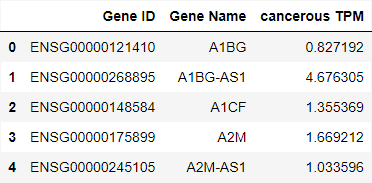
\includegraphics[height=\dfheight]{figures/03_01_CMP_cancer_mean}
    \caption{Example data of processed Cell Modell Passport dataset}
    \label{fig:03_01_df_CMP_cancer_mean}
\end{figure}

